\documentclass[12pt,titlepage]{article}
\usepackage[utf8]{inputenc}
\usepackage[T1]{fontenc}
\usepackage[english]{babel}
\usepackage[a4paper]{geometry}
\frenchspacing
\usepackage{amsfonts}
\usepackage{amsmath}
\usepackage{amssymb}
\usepackage{amsthm}
\usepackage{setspace}
\usepackage{fullpage}
\usepackage{tocbibind}
\usepackage{graphicx}
\usepackage{url}
\usepackage{verbatim}
\usepackage{listings}
%\usepackage{gitinfo2}
\usepackage{hyperref}
\usepackage{cleveref}
\usepackage{cite}
\usepackage{color}
\usepackage{enumitem}
\usepackage{usecases}
\usepackage{nameref}

\definecolor{pblue}{rgb}{0.13,0.13,1}
\definecolor{pgreen}{rgb}{0,0.5,0}
\definecolor{pred}{rgb}{0.9,0,0}
\definecolor{pgrey}{rgb}{0.46,0.45,0.48}
\lstset{language=Java,
  showspaces=false,
  showtabs=false,
  breaklines=true,
  showstringspaces=false,
  breakatwhitespace=true,
  commentstyle=\color{pgreen},
  keywordstyle=\color{pblue},
  stringstyle=\color{pred},
  basicstyle=\ttfamily,
  moredelim=[il][\textcolor{pgrey}]{$$},
  moredelim=[is][\textcolor{pgrey}]{\%\%}{\%\%}
}
\renewcommand{\labelitemi}{$\bullet$}
\renewcommand{\labelitemii}{$\cdot$}
\renewcommand{\labelitemiii}{$\diamond$}
\renewcommand{\labelitemiv}{$\ast$}


\begin{document}
\title{
	Design Document for Bicycle Garage Pro\\
	(Group 33, 2015)\\
	\vspace{0.2in}
	\normalsize Current version: 0.9.1
}
\author{
	Alexander Skafte\\
	\url{tfy13ask@student.lu.se}\\
	Dennis Jin\\
	\url{desuvader@gmail.com}\\
	Petter Berntsson\\
	\url{dat14pbe@student.lu.se}\\
	Emelie Löthman\\
	\url{pol14elo@student.lu.se}\\
	Adam Mzrozek\\
	\url{dat14amr@student.lu.se}
}
\date{}



\maketitle
\newpage
\tableofcontents
\thispagestyle{empty}
\setcounter{page}{0}
\newpage

% ----- REFERENCES & -----------------------------------------------------------
% ----- BIBLIOGRAPHY -----------------------------------------------------------

\section{References}
\label{sec:references}

\begin{itemize}
	\item \textit{Examples and Exercises in the Software
		Engineering Process}. ETSA01 VT 2015. Deparment of Computer
		Science, Lund University. March 10, 2015.
	\item \textit{Software Requirements Specification for Bicycle Garage
		Pro}. ETSA01, Group 33, 2015.
\end{itemize}

% ----- INTRODUCTION -----------------------------------------------------------

\section{Introduction}
\label{sec:introduction}

\subsection{Tested system}
\label{subsec:tested-system}

The system described in this document is the software for a public bicycle
garage. This software is responsible for managing the authentication of users
and the management of their information and their bicycles.

This document provides a specification for testing the bicycle garage software.
The test process consists of the following phases:

\begin{itemize}
	\item Unit testing
	\item System testing
	\item Acceptance testing
\end{itemize}

% ----- TEST PROCESS -----------------------------------------------------------

\section{Test process}
\label{sec:test-process}

\subsection{Process overview}
\label{subsec:test-process-process-overview}

The tests of the software are carried out on several levels of abstraction:

\begin{itemize}
\item
At the lowest level, \textit{unit testing} is performed which aim to test each
line of code inside the software.
\item
These units are grouped into modules, which would
normally be tested through the API or \textit{Application Programming
Interface}, a process known as \textit{integration testing}. For this software
however, integration testing will not be performed due to the smallness of the
software.
\item
On an even higher level of abstraction, so called \textit{system testing} is
performed which ensures that the requirements provided in the \textit{Software
Requirements Specification} are fulfilled.
\item
Lastly, \textit{acceptance testing} is performed. However, acceptance
testing is performed by the customer and thus not within the scope of this
document.
\end{itemize}

\subsection{Unit testing}
\label{subsec:test-process-unit-testing}

Unit testing aims to test each line of software code. Every non-trivial function
is tested in software through the use of a test suite library.

\begin{description}
	\item[Performed by:]	Developers
	\item[Type of test:]	Structural
	\item[Criteria:]	Every important line of code is tested
	\item[Stop rule:]	No errors found
\end{description}


%
%\subsection{Integration testing}
%\label{subsec:test-process-integration-testing}
%
%Integration testing is performed in a similar way to unit testing, but larger
%and more inclusive modules are tested. Each module is tested in software through
%the use of a test suite library.
%
%\begin{description}
%	\item[Performed by:]	Developers
%	\item[Type of test:]	Structural
%	\item[Criteria:]	Every API method is tested completely
%	\item[Stop rule:]	No errors found
%\end{description}
%

\subsection{System testing}
\label{subsec:test-process-system-testing}

During system testing, all requirements specified inside the \textit{Software
Requirements Specification} are tested.

\begin{description}
	\item[Performed by:]	Developers
	\item[Type of test:]	Functional
	\item[Criteria:]	All requirements inside the SRS are fulfilled
	\item[Stop rule:]	No critical errors found
\end{description}

\subsection{Acceptance testing}
\label{subsec:test-process-acceptance-testing}

Acceptance testing is performed by the client and not by the developers, and is
thus not discussed in this document.

% ----- TESTED ITEMS -----------------------------------------------------------

\section{Tested items}
\label{sec:tested-items}

TODO \\

... perhaps this section should be removed? In the example found in the green
booklet for the course, this section is nothing but a repetition of what has
already been said.


% ----- TEST RECORDING PROCEDURE -----------------------------------------------

\section{Test recording procedure}
\label{sec:test-recording-procedure}

\subsection{Unit testing}
\label{subsec:test-recording-procedure-unit-testing}

Every non-trivial piece of software code is tested individially by the
developers. These tests are automated and performed incrementally as the
code base grows. The results of these tests do not have to be recorded; the
rationale for this being that the tests provide enough assurance on their own
and that the size of the test log would soon grow out of hand.

%
%\subsection{Integration testing}
%\label{subsec:test-recording-procedure-integration-testing}
%

\subsection{System testing}
\label{subsec:test-recording-procedure-system-testing}

For each test session carried out, a new requirements coverage matrix shall be
produced according to the one shown in \textit{Appendix \ref{app:RCM}:
Requirements Coverage Matrix}. In a document containing this matrix, the result
of each test case shall be displayed. Any faults found shall be reported to the
developers, either directly or through the use of a shared file where error
reports are logged.

\subsection{Acceptance testing}
\label{subsec:test-recording-procedure-acceptance-testing}

Acceptance testing is performed by the client and not by the developers, and is
thus not discussed in this document.


% ----- TEST CASES FOR SYSTEM TESTING ------------------------------------------

\section{Test cases for system testing}
\label{sec:test-cases-for-system-testing}

\subsection{Test cases}
\label{subsec:test-cases}

Since unit testing is performed in the software environment and acceptance
testing is performed by the customer, only system testing will be fully
described in this document. For this purpose, please refer to
\textit{Appendix \ref{app:test-cases}: \nameref{app:test-cases}}.

\subsection{Requirements coverage and traceability}
\label{subsec:requirements-coverage-and-testability}

All functional requirements provided in the \textit{Software Requirements
Specification} should be tested by at least on test case to ensure that all
functionality is tested. For this purpose, a \textit{requirements coverage
matrix} is used. For this matrix, please refer to \textit{Appendix
\ref{app:RCM}: Requirements Coverage Matrix}.


% ----- APPENDIX ---------------------------------------------------------------
% ------------- Test Cases -----------------------------------------------------

\newpage
\appendix

\section{Test cases}
\label{app:test-cases}

\begin{usecase}
	\addtitle{Test case 1:}{Registration of a new user}
	\addfield{Primary actor:}{Operator}
	\addfield{Preconditions:}{User is unregistered}
	\addfield{Postconditions:}{User is registered}
	\addscenario{Main success scenario:}{
		\item The operator provides the required user information to the
			control interface.
		\item A new PIN code is generated for the user.
		\item The user is added to the system.
	}
\end{usecase}

\begin{usecase}
	\addtitle{Test case 2:}{Registration of an already registered user}
	\addfield{Primary actor:}{Operator}
	\addfield{Preconditions:}{User is registered}
	\addfield{Postconditions:}{User is registered}
	\addscenario{Main success scenario:}{
		\item The operator provides the required user information to the
			control interface.
		\item The system responds with an error message, e.g. ''The user
			is already registered.''
	}
\end{usecase}

\begin{usecase}
	\addtitle{Test case 3:}{Unregistration of a registered user}
	\addfield{Primary actor:}{Operator}
	\addfield{Preconditions:}{User is registered}
	\addfield{Postconditions:}{User is unregistered}
	\addscenario{Main success scenario:}{
		\item The operator provides the required user information to the
			control interface.
		\item All bicycles associated with the user are removed from the
			system.
		\item The user is removed from the system.
	}
\end{usecase}

\begin{usecase}
	\addtitle{Test case 4:}{Association of a new bicycle with a user}
	\addfield{Primary actor:}{Operator}
	\addfield{Preconditions:}{User is registered; garage is not full}
	\addfield{Postconditions:}{Bicycle is associated with user}
	\addscenario{Main success scenario:}{
		\item The operator provides the required user information to the
			control interface.
		\item A unique 5-digit identification number is generated and
			associated with the bicycle.
		\item The bicycle is added to the set of bicycles owned by the
			user.
		\item A barcode associated with the 5-digit ID is printed and
			given to the user.
	}
\end{usecase}

\begin{usecase}
	\addtitle{Test case 5:}{Disassociation of a user's bicycle}
	\addfield{Primary actor:}{Operator}
	\addfield{Preconditions:}{The user is registered. The bicycle is
					associated with the user.}
	\addfield{Postconditions:}{Bicycle is not associated with user nor is it
					present in the system.}
	\addscenario{Main success scenario:}{
		\item The operator provides the required user information to the
			control interface.
		\item The bicycle is disassociated with the user.
		\item The unique 5-digit identification number associated with
			the bicycle is returned to the pool of available ID's.
			As a consequence, the barcode is rendered invalid.
	}
\end{usecase}

\begin{usecase}
	\addtitle{Test case 6:}{A valid PIN code is entered}
	\addfield{Primary actor:}{User}
	\addfield{Preconditions:}{The PIN code entered is associated with a
					registered user, who has at least
					one bicycle stored in the garage.}
	\addfield{Postconditions:}{-}
	\addscenario{Main success scenario:}{
		\item User enters their PIN code at the PIN code terminal.
		\item The green LED lamp is lit for 4 seconds. Simultaneously,
			the entrance door opens and stays open for 10 seconds.
	}
\end{usecase}

\begin{usecase}
	\addtitle{Test case 7:}{An invalid PIN code is entered}
	\addfield{Primary actor:}{User}
	\addfield{Preconditions:}{The PIN code entered is not associated with
					any registered user.}
	\addfield{Postconditions:}{-}
	\addscenario{Main success scenario:}{
		\item User enters the PIN code at the PIN code terminal.
		\item The red LED lamp is lit for 4 seconds. 
	}
\end{usecase}

\begin{usecase}
	\addtitle{Test case 8:}{Recovery of a lost/forgotten PIN code}
	\addfield{Primary actor:}{Operator}
	\addfield{Preconditions:}{The user is registered.}
	\addfield{Postconditions:}{-}
	\addscenario{Main success scenario:}{
		\item The operator provides the required user information to the
			control interface.
		\item The operator requests the PIN code from the system, and
			gives it to the user.
	}
\end{usecase}

\begin{usecase}
	\addtitle{Test case 9:}{Modification of a user's PIN code}
	\addfield{Primary actor:}{Operator}
	\addfield{Preconditions:}{The user is registered and there are available
					PIN codes left.}
	\addfield{Postconditions:}{The user's PIN code is updated.}
	\addscenario{Main success scenario:}{
		\item The operator provides the required user information to the
			control interface.
		\item The operator asks the system to generate a new PIN code.
		\item A PIN code is successfully generated and associated with
			the user.
	}
\end{usecase}

\begin{usecase}
	\addtitle{Test case 10:}{An invalid PIN code is entered}
	\addfield{Primary actor:}{User}
	\addfield{Preconditions:}{The PIN code entered is not associated with
					any registered user.}
	\addfield{Postconditions:}{-}
	\addscenario{Main success scenario:}{
		\item User enters the PIN code at the PIN code terminal.
		\item The red LED lamp is lit for 4 seconds. 
	}
\end{usecase}

\begin{usecase}
	\addtitle{Test case 11:}{An invalid barcode is scanned}
	\addfield{Primary actor:}{User or other person}
	\addfield{Preconditions:}{The barcode is not a part of the system.}
	\addfield{Postconditions:}{-}
	\addscenario{Main success scenario:}{
		\item The invalid barcode is scanned.
		\item The red LED lamp is lit for 4 seconds. 
	}
\end{usecase}

\begin{usecase}
	\addtitle{Test case 12:}{Creation of a new barcode for an existing
					bicycle}
	\addfield{Primary actor:}{Operator}
	\addfield{Preconditions:}{The user is registered and the subject bicycle
					is associated with them.}
	\addfield{Postconditions:}{A new barcode is associated with the subject
					bicycle's 5-digit identification
					number.}
	\addscenario{Main success scenario:}{
		\item The operator provides the required user information,
			including the bicycle's 5-digit identification number,
			to the control interface.
		\item The old barcode associated with the ID is rendered invalid
			and a new one is generated, associated with the ID and
			then printed.
	}
\end{usecase}

\newpage

\section{Requirements Coverage Matrix}
\label{app:RCM}

In the requirements coverage matrices shown below, requirements are shown on the
vertical axes and test cases on the horizontal axes.

\begin{figure}[H]
	\centering
	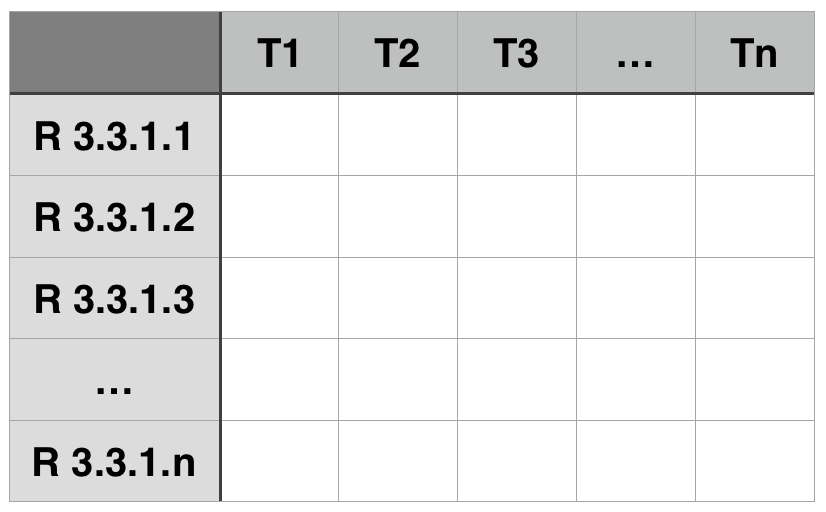
\includegraphics[width=0.5\textwidth]{./assets/rcm-empty.png}
	\caption{A minimal example of an empty requirements coverage matrix.}
	\label{fig:rcm-empty}
\end{figure}

\begin{figure}[H]
	\centering
	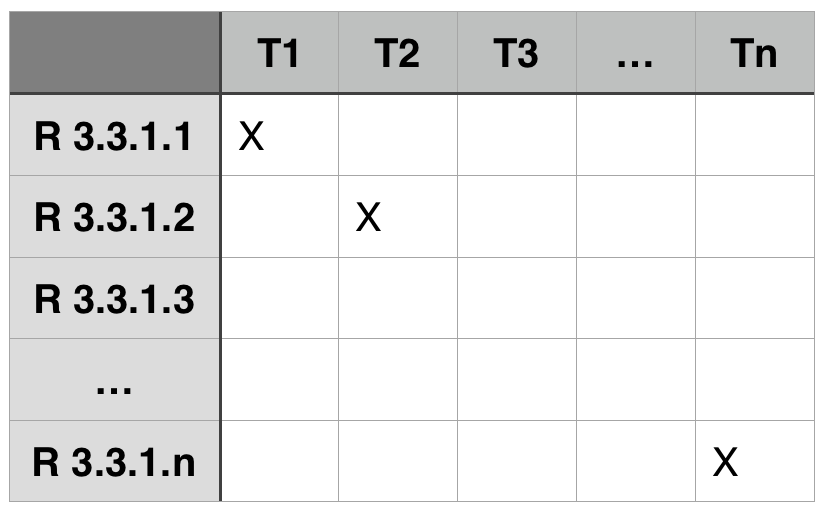
\includegraphics[width=0.5\textwidth]{./assets/rcm-incomplete.png}
	\caption{A minimal example of partly filled requirements coverage
		matrix.}
	\label{fig:rcm-incomplete}
\end{figure}

\begin{figure}[H]
	\centering
	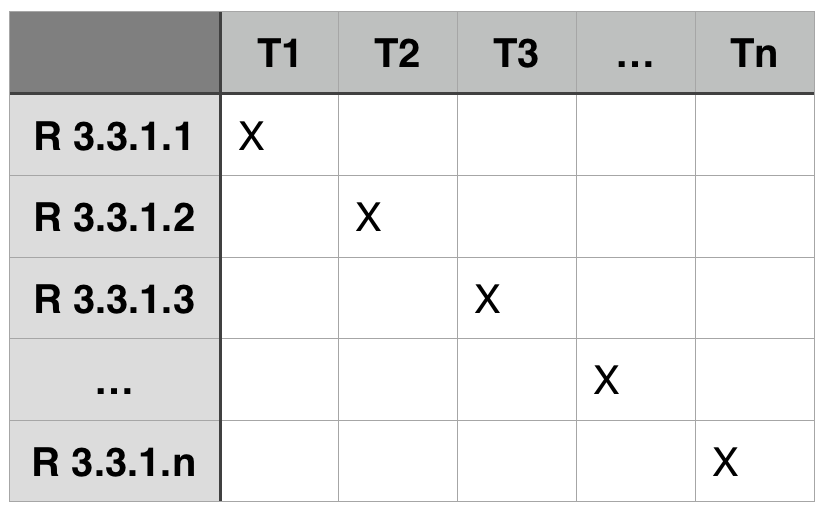
\includegraphics[width=0.5\textwidth]{./assets/rcm-filled.png}
	\caption{A minimal example of a filled requirements coverage matrix.}
	\label{fig:rcm-filled}
\end{figure}

\end{document}

